%!tex program=xelatex
\documentclass[12pt]{article}
% \usepackage{ctex}
\usepackage{CJK}
\usepackage{subfigure}

\usepackage{fancyhdr}
\usepackage{booktabs}
\usepackage{longtable}
\usepackage{tabularx}
\usepackage{multirow}
\usepackage{threeparttable}
\usepackage{titlesec}
\usepackage{graphicx}
\usepackage{float}
\usepackage{amsmath, amsfonts, amssymb, amsthm}
\usepackage{algorithm, algorithmic}
\usepackage{hyperref}
\usepackage{makeidx}\makeindex
\usepackage{geometry}[top=20mm, bottom=20mm, left=20mm, right=20mm]
\usepackage[dvipsnames, svgnames, x11names]{xcolor}
\usepackage{listings}
\lstset{
    language = c++,
    backgroundcolor     =   \color{WhiteSmoke},
    basicstyle          =   \sffamily,
    keywordstyle        =   \bfseries,
    commentstyle        =   \rmfamily\itshape,
    stringstyle         =   \ttfamily,
    flexiblecolumns,
    numbers             =   left,   % 行号的位置在左边
    showspaces          =   false,  % 是否显示空格,显示了有点乱,所以不现实了
    numberstyle         =   \ttfamily\tiny,    % 行号的样式,小五号,tt等宽字体
    showstringspaces    =   false,
    captionpos          =   t,      % 这段代码的名字所呈现的位置,t指的是top上面
    % frame               =   lrtb,   % 显示边框
    keywordstyle        =   \color{SlateGray},
    breaklines          =   true,   % 自动换行,建议不要写太长的行
    %columns             =   fixed,  % 如果不加这一句,字间距就不固定,很丑,必须加
}


% \lstdefinestyle{C++}{
%     language        =   C,
%     basicstyle      =   \zihao{-5}\ttfamily,
%     numberstyle     =   \zihao{-5}\ttfamily,
%     keywordstyle    =   \color{blue},
%     keywordstyle    =   [2] \color{teal},
%     stringstyle     =   \color{magenta},
%     commentstyle    =   \color{red}\ttfamily,
%     breaklines      =   true,   % 自动换行,建议不要写太长的行
%     columns         =   fixed,  % 如果不加这一句,字间距就不固定,很丑,必须加
%     basewidth       =   0.5em,
% }
\usepackage{verbatim}

\title{Chap3 Interpolation and Polynomial Approximation}
\author{Xu Feng, imxufeng@outlook.com, 201900090026}
\date{\today}

\begin{document}

% \Large

\maketitle

\section{Introduction}

As Weierstrass approximation theorem, any function $f$ can be approximated by polynomials. In this work, I review several polynomial interpolation methods illustrated in the book \cite{1} with C++ implementations, including Lagrange, Neville, Newton and Hermite's method, followed with analysis and comparison of different methods. Detailed interpolation and experiment codes is shown in the appendix.

\section{Implementations of polynomial class}

Operations of add and multiply of polynomials are needed in the implementation of interpolation methods, but there is no existing polynomial class in Standard Template Library of C++. So the first thing to do is to form a polynomial class which includes overloaded operators of add and multiply.

Implementations of polynomial class is in the file ``poly.h''. The constructor of the poly class can be made of a vector of double denoting the coefficients of the polynomial, which is the basis of following overloaded operators.

With $ f(x) = \sum_{i=0}^{n} a_i x^i$ and $g(x) = \sum_{i=0}^{m} b_i x^i$, we have:
 $$f(x)+g(x)=\sum_{i=0}^{max(n,m)}(a_i+b_i)x^i, $$ and:
$$ f(x)g(x) = \sum_{k=0}^{n+m}(\sum_{i=0}^{k} a_i b_{k-i}) x^k. $$

It is possible that after the operations like add or multiply, several coefficient of the vector will be zero, especially the highest term of the polynomial in which case the degree of the polynomial should be updated. For example, take $f(x)=1+2x+3x^2$ with degree of two and $g(x)=1+x-3x^2$ with degree of two, but $f(x)+g(x)=2+3x$ with degree 3 which is less than two. If not checked, bugs will be raised in the following implementation process.

With above analysis, I implement the poly class with C++, detailed codes can be found in Appendix \ref{codePoly}.

\section{Different methods and comparison}
The polynomial methods can be categoried into two classes, one is the n-th degree polynomial result given n+1 data point and corresponding value of the function, and the other is (2n+1)-th degree polynomial result with extra knowledge of the derivative values of the given data point. Implementation codes can be found in Appendix \ref{codeInter}.

\subsection{Polynomial interpolation of degree n}

\subsubsection{Similarity and difference}
Lagrange, Neville and Newton's divided difference methods give the same result as these three methods all assume that the expected form the polynomial is the one with degree n, which gives the unique solution given the same data.

Lagrange method gives a explicit formula of the polynomial given data points, while Neville and Newton are both iterated algorithm which give the same result as Lagrange but calculate in a different way.

\subsection{Prediction with data in the book}
We use the data of 3c on page 110 the book \cite{1}, which gives that the point is $0.1, 0.2, 0.3, 0.4$, and the function value is 0.62049958, -0.28398668, 0.00660095, 0.24842440. The task is to predict f(0.25).

The result is the interpolation polynomial $p(x)=(3.9639)+(-49.7747)x^1+(184.138)x^2+(-207.306)x^3$ and $p(0.25)=-0.210337$ gives an approximation of $f(0.25)$.

\subsubsection{Experiments of efficiency}

The efficiency of the three algorithms is highly related to the property of given data. The following figure is a comparison of running time among these three algorithms. The experiment data is based on serval points with the corresponding function values randomly generated, and we takes the average running time of 100 repeats. We take the data points between 0 and 1, and also check points range from 0 to maximum of interger. It is found that different experiments get different results. The x label is the number of points and the y label is running time for 10 repeats.

\begin{figure}[!h]
    \centering
    
    \subfigure[Running time of data points ranging from 0 to 1 (repeat 10 times)]{
    \begin{minipage}[t]{0.45\linewidth}
    \centering
    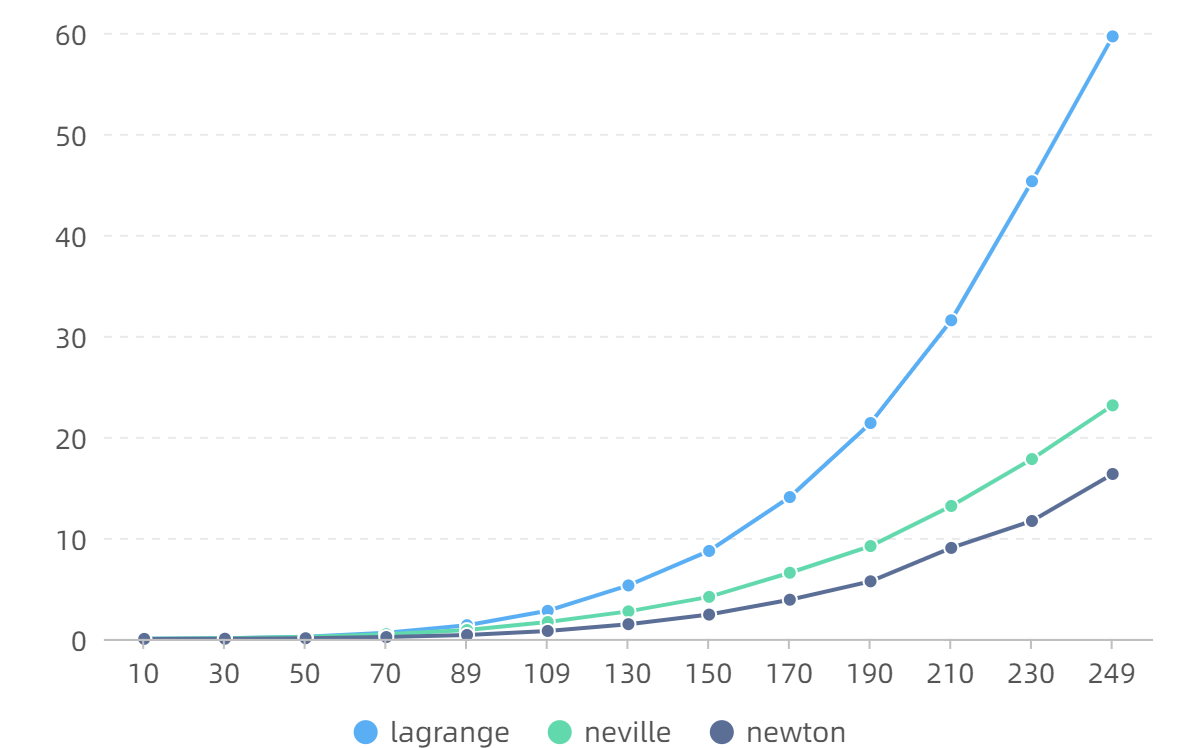
\includegraphics[width=\textwidth]{small.png}
    %\caption{fig1}
    \end{minipage}%
    }%
    \subfigure[Running time of data points with larger range (repeat 10 times)]{
    \begin{minipage}[t]{0.45\linewidth}
    \centering
    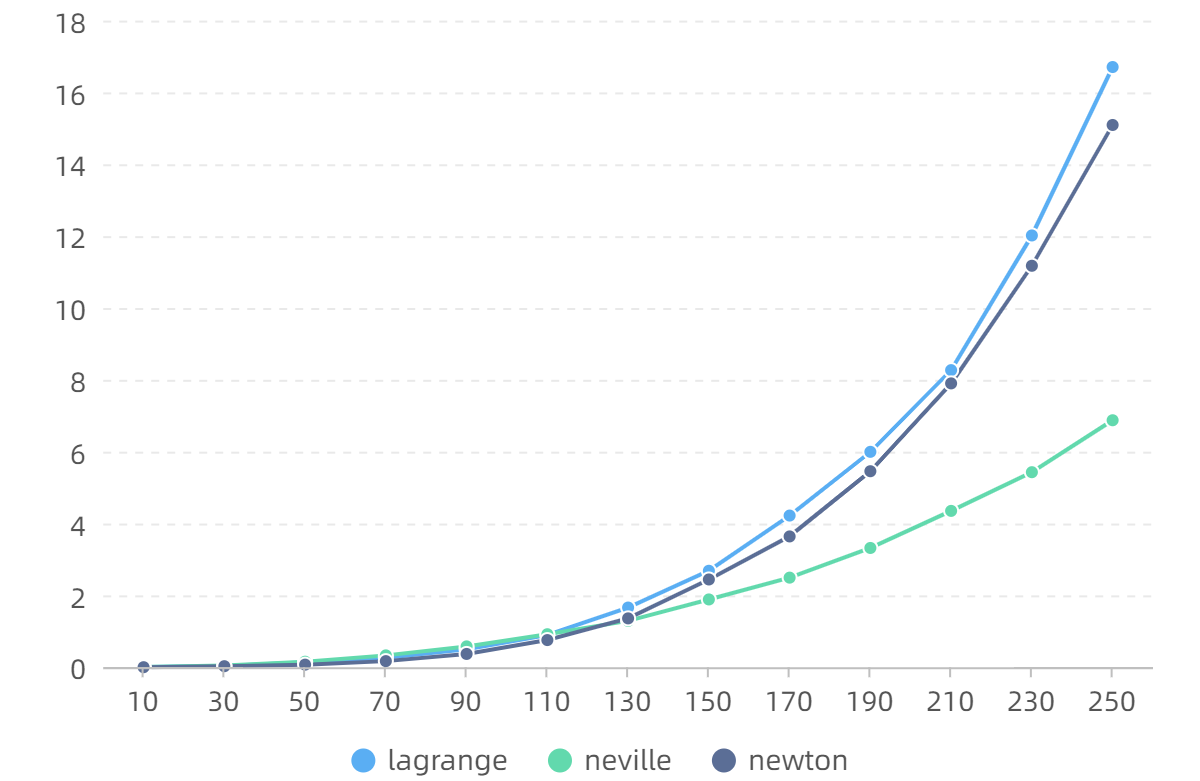
\includegraphics[width=\textwidth]{large.png}
    %\caption{fig2}
    \end{minipage}%
    }%
\end{figure}

In the former experiment, the points are all between 0 and 1,the nature of explicit formula brings Lagrange polynomial interpolation too much things to calculate, and as a result, it may take much more time than the other two. As the data points are all between 0 and 1, Neville and Newton's method shows great superiority in the performance of calculating.

But when the range of points become larger, things become different. It is shown in the right figure that when the number of points become larger, Newton's method gets worse, while Neville's method perfomrs better.


\subsection{Polynomial interpolation of degree 2n+1}

With the knowledge of derivative values of given data point, we can get the result of polynomial of degree 2n+1 by the algorithm of Hermite. Hermite's algorithm can also implemented in a divided difference way.

We use the data of 1d on page 139 the book \cite{1}, which gives that the point is $0.1, 0.2, 0.3, 0.4$, and the function value is -0.62049958, 0.28398668, 0.00660095, 0.24842440. Also the derivative is known as 3.58502082, 3.14033271, 2.66668043, 2.16529366, respectively.

The result is the interpolation polynomial of degree n is $p_0(x)=(-4.40794)+(57.9594)x^1+(-229.202)x^2+(283.514)x^3$, and the (2n+1)-th degree polynomial is $p_1(x)=(-21.447)+(855.96)x^1+(-14329.1)x^2+(125096)x^3+(-610571)x^4+(1.67552e+06)x^5+(-2.41389e+06)x^6+(1.41993e+06)x^7$. The approximation of $f(0.25)$ is $p_0(0.25)=0.18671$ and $p_1(0.25)=0.136794$.

\subsection{Comparison between degree n method and degree 2n+1 method}

What can be explicitly seen in Taylor's theorem is that higher degree polynomial may have higher posssibility to approximate the function.

Take $f(x)=e^{x}$ as an example. We give $x=1,2,3,4$ and $f(x)=exp(1),exp(2),exp(3),exp(4)$ respectively for these algorithms and give $f'(x)=exp(1),exp(2),exp(3),exp(4)$ as an extra knowledge for method Hermite.

We get the result that: the first three algorithms give $p_0(x)=(-7.71721)+(17.9147)x^1+(-9.77757)x^2+(2.2984)x^3$, while Hermite gives that $p_1(x)=(0.856415)+(1.58543)x^1+(-0.489549)x^2+(1.06998)x^3+(-0.443636)x^4+(0.163895)x^5+(-0.0268424)x^6+(0.00259051)x^7$.

We test on value 6, and get that $p_0(6)=244.233$ and $p_1(6)=396.173$, while the ground truth is that $exp(6)=403.429$. We also test on value 2.5, which is between the minimum number 1 and the maximum number of 4, and find that $p_0(x)=11.8722$ and $p_1(x)=12.1824$, while the ground truth is $exp(6)=12.1825$.

It is obvious from the above example that in most times Hermite interpolation method gives higher-degree polynomial, which reduces the error and gets better interpolation performance.

\section{Conclusion}

Different polynomial interpolation methods have their own superiority faced with different situations. Usually 

\begin{thebibliography}{99}
\bibitem{1} Burden, Richard L., J. Douglas Faires, and Annette M. Burden. Numerical analysis. Cengage learning, 2015.

\end{thebibliography}

\appendix

\section{Codes: CMakeLists.txt}

\begin{lstlisting}
cmake_minimum_required(VERSION 3.21)
project(cm3)

set(CMAKE_CXX_STANDARD 14)

add_executable(cm3 poly.h main.cpp test3.h interpolation.h)
\end{lstlisting}

\section{Codes: Poly.h}\label{codePoly}
\begin{lstlisting}{cpp}
#ifndef CM3_POLY_H
#define CM3_POLY_H

#include <vector>
#include <cmath>
using std::vector, std::cin, std::cout, std::endl, std::pow;

class DivByZeroException : public std::exception{
public:
    [[nodiscard]] const char * what () const noexcept override {
        return "DivByZero";
    }
};

class Poly {
public:
    Poly(){
        this->deg = 0;
        this->coefs = vector<double>{1.};
    }
    Poly(double m){
        this->deg = 0;
        this->coefs = vector<double>{m};
    }
    Poly(vector<double> coefs){
        this->deg = coefs.size()-1;
        this->coefs = coefs;
    }
    int getDeg() const{
        return this->coefs.size()-1;
    }
    double getCoef(int i) const{
        return this->coefs[i];
    }
    vector<double> getCoefs() const{
        return this->coefs;
    }
    void print() const{
        cout << "(" << this->coefs[0] << ")";
        for(int i=1; i<this->coefs.size(); i++){
            cout << "+(" << this->coefs[i] << ")x^" << i;
        }
        cout << endl;
    }
    double getValue(double x){
        double res = 0.;
        for(int i=0; i<=getDeg(); i++){
            res += getCoef(i) * std::pow(x, i);
        }
        return res;
    }
private:
    int deg = -1;
    vector<double> coefs;
};


Poly operator+(Poly const& p0, Poly const& p1){
    vector<double> res;
    double tmp;
    int deg;
    for(int i=0; i<std::max(p0.getDeg(), p1.getDeg())+1; i++) {
        tmp = 0.;
        if (i <= p0.getDeg()) tmp += p0.getCoef(i);
        if (i <= p1.getDeg()) tmp += p1.getCoef(i);
        res.push_back(tmp);
        if (std::abs(tmp)>=1e-10) {deg = i;}
    }
    for(int i=deg+1; i<std::max(p0.getDeg(), p1.getDeg())+1; i++) {
        res.pop_back();
    }
    return {res};
}

Poly operator*(Poly const& p0, Poly const& p1){
    vector<double> res;
    double tmp = 0.;
    int deg;
    for(int i=0; i<=p0.getDeg()+p1.getDeg(); i++){
        tmp = 0.;
        for(int j=0; j<=i; j++){
            if (j<=p0.getDeg() && i-j<=p1.getDeg()) {
                tmp += p0.getCoef(j) * p1.getCoef(i - j);
            }
        }
        if (std::abs(tmp)>=1e-10) {deg = i;}
        res.push_back(tmp);
    }
    for(int i=deg+1; i<std::max(p0.getDeg(), p1.getDeg())+1; i++) {
        res.pop_back();
    }
    return {res};
}

Poly operator*(Poly const& p0, double m) {
    vector<double> res;
    for(int i=0; i<=p0.getDeg(); i++){
        res.push_back(p0.getCoef(i)*m);
    }
    return {res};
}


Poly operator/(Poly const& p0, double m){
    if (std::abs(m)<1e-20) throw DivByZeroException();
    vector<double> res;
    for(int i=0; i<=p0.getDeg(); i++){
        res.push_back(p0.getCoef(i)/m);
    }
    return {res};
}


Poly operator-(Poly& p0, double m){
    vector<double> res = p0.getCoefs();
    res[0] -= m;
    return {res};
}


Poly operator+(Poly& p0, double m){
    vector<double> res = p0.getCoefs();
    res[0] += m;
    return {res};
}

#endif //CM3_POLY_H
\end{lstlisting}
\section{Codes: interpolation.h}\label{codeInter}
\begin{lstlisting}{c++}

#ifndef CM3_INTERPOLATION_H
#define CM3_INTERPOLATION_H

#include "poly.h"
#include <vector>
#include <iostream>
using std::vector, std::cout, std::cin, std::endl;


class LengthMatch : std::exception {
public:
    [[nodiscard]] const char * what () const noexcept override {
        return "Length does not match!";
    }
};

class Interpolation {
public:
    static Poly lagrange(vector<double> xList, vector<double> yList){
        try{
            if (xList.size() != yList.size()) throw LengthMatch();
            int n = xList.size()-1;
            Poly p = vector<double> {0.};
            for (int k=0; k<=n; k++){
                Poly lnk = vector<double> {1.};
                for (int i=0; i<=n; i++){
                    if (i != k){
                        Poly x = vector<double> {-xList[i], 1.};
                        Poly tmp =  x / (xList[k] - xList[i]);
                        lnk = lnk * tmp;
                    }
                }
                Poly tmp = lnk * yList[k];
                p = p + tmp;
            }
            return p;
        }
        catch (LengthMatch& lengthMatch){
            cout << lengthMatch.what() << endl;
        }
    }

    static Poly neville(vector<double> xList, vector<double> yList){
        try{
            const int n = xList.size()-1;
            Poly Q[n+1][n+1];
            for(int i=0; i<=n; i++){
                Q[i][0] = Poly(vector<double>{yList[i]});
            }

            for(int i=1; i<=n; i++){
                for(int j=1; j<=i; j++){
                    Q[i][j] = (Poly(vector<double>{-xList[i-j], 1.}) * Q[i][j-1]
                            + Poly(vector<double>{-xList[i], 1.}) * Q[i-1][j-1] * (-1.))
                                    /(xList[i]-xList[i-j]) ;
                }
            }
            return Q[n][n];
        }
        catch (LengthMatch& lengthMatch){
            cout << lengthMatch.what() << endl;
        }
    }

    static Poly newton(vector<double> xList, vector<double> yList){
        try{
            const int n = xList.size()-1;
            double F[n+1][n+1];

            for(int i=0; i<=n; i++){
                F[i][0] = yList[i];
            }

            for(int i=1; i<=n; i++){
                for(int j=1; j<=i; j++){
                    F[i][j] = (F[i][j-1]-F[i-1][j-1])/(xList[i]-xList[i-j]);
                }
            }

            Poly p = Poly(F[0][0]);

            Poly tmp;
            for(int i=1; i<=n; i++){
                tmp = Poly(1.);
                for(int j=0; j<=i-1; j++){
                    tmp = tmp * Poly(vector<double>{-xList[j], 1.});
                }
                tmp = tmp * F[i][i];
                p = p + tmp;
            }
            return p;
        }
        catch (LengthMatch& lengthMatch){
            cout << lengthMatch.what() << endl;
        }
    }

    static Poly hermite(vector<double> xList, vector<double> yList, vector<double> deList){
        try {
            const int n = xList.size()-1;
            double z[2*n+2];
            double Q[2*n+2][2*n+2];

            for (int i = 0; i <= n; i++) {
                z[2*i] = xList[i];
                z[2*i+1] = xList[i];
                Q[2*i][0] = yList[i];
                Q[2*i+1][0] = yList[i];
                Q[2*i+1][1] = deList[i];

                if(i != 0){
                    Q[2*i][1] = (Q[2*i][0]-Q[2*i-1][0])/(z[2*i]-z[2*i-1]);
                }
            }

            for(int i=2; i<=2*n+1; i++){
                for(int j=2; j<=i; j++){
                    Q[i][j] = (Q[i][j-1]-Q[i-1][j-1])/(z[i]-z[i-j]);
                }
            }

            Poly h = Poly(Q[0][0]);
            Poly tmp = Poly(1.);
            for(int i=1; i<=n; i++){
                tmp = tmp * Poly(vector<double>{-xList[i-1], 1.});
                h = h + tmp * Q[2*i-1][2*i-1];
                tmp = tmp * Poly(vector<double>{-xList[i-1], 1.});
                h = h + tmp * Q[2*i][2*i];
            }
            tmp = tmp * Poly(vector<double>{-xList[n], 1.});
            h = h + tmp * Q[2*n+1][2*n+1];
            return h;

        }
        catch (LengthMatch& lengthMatch){
            cout << lengthMatch.what() << endl;
        }
    }

};

#endif //CM3_INTERPOLATION_H
    
\end{lstlisting}

\section{Codes: experiments and plots}
\begin{lstlisting}
#include <iostream>
#include <vector>
#include <ctime>
#include "test3.h"
#include "interpolation.h"
#include <functional>
#include <algorithm>
using std::vector, std::cout, std::cin, std::exp, std::sort;

template<typename F>
double recordTime(F f, int repeat = 1){
    std::clock_t t;
    t = std::clock();
    for (int repeat_ = 0; repeat_ < repeat; repeat_++){
        auto&& res = f();
    }
    t = std::clock() - t;
    cout<<(double)(t)/CLOCKS_PER_SEC<<",";
    return (double)(t)/CLOCKS_PER_SEC;
}

static double f(double x) { return exp(x); }
static double f1(double x) { return exp(x); }

int main() {

//    // generate random data to test efficiency
//    for(int len=10; len<=500; len+=20){
//        cout << len << ",";
//        vector<double> xList4;
//        vector<double> yList4;
//        for (int i=0; i<len; i++){
//            xList4.push_back(((double) rand() / (RAND_MAX)));
//            sort(xList4.begin(), xList4.end());
//            xList4.erase(unique(xList4.begin(), xList4.end()), xList4.end());
//        }
//
//        cout << xList4.size() << ",";
//
//        for (int i=0; i<xList4.size(); i++){
//            yList4.push_back(((double) rand() / (RAND_MAX)));
//        }
//        int repeat = 10;
//        recordTime([xList4, yList4]{return Interpolation::lagrange(xList4, yList4);}, repeat);
//        recordTime([xList4, yList4]{return Interpolation::neville(xList4, yList4);}, repeat);
//        recordTime([xList4, yList4]{return Interpolation::newton(xList4, yList4);}, repeat);
//
//        cout << endl;
//    }


//    vector<double> xList = {1., 2., 3., 4.};
//    vector<double> yList = {1., 4., 9., 16.};
//    vector<double> deList = {2., 4., 6., 8.};

//    vector<double> xList = {1., 2., 3., 4.,};
//    vector<double> yList = {f(1.), f(2.), f(3.), f(4.)};
//    vector<double> deList = {f1(1.), f1(2.), f1(3.), f1(4.)};

    // p119 3c
//    vector<double> xList = {0.1, 0.2, 0.3, 0.4};
//    vector<double> yList = {0.62049958, -0.28398668, 0.00660095, 0.24842440};

    // p139 1d
    vector<double> xList = {0.1, 0.2, 0.3, 0.4};
    vector<double> yList = {-0.62049958, 0.28398668, 0.00660095, 0.24842440};
    vector<double> deList = {3.58502082, 3.14033271, 2.66668043, 2.16529366};

    Poly p0 = Interpolation::lagrange(xList,yList);
    Poly p1 = Interpolation::neville(xList, yList);
    Poly p2 = Interpolation::newton(xList, yList);
    Poly p3 = Interpolation::hermite(xList, yList, deList);

    p0.print();
    p1.print();
    p2.print();
    p3.print();

//    cout << p0.getValue(6) << endl;
//    cout << p0.getValue(2.5) << endl;
//    cout << p3.getValue(6) << endl;
//    cout << p3.getValue(2.5) << endl;
//    cout << f(6) << endl;
//    cout << f(2.5) << endl;

    cout << p0.getValue(0.25) << endl;
    cout << p3.getValue(0.25) << endl;




}
\end{lstlisting}
\end{document}
